
After a set of possible solutions with the frequency controllers have been proposed, now an approach in the state-space domain is provided. This is possible thanks to the estimations made through the \textit{greyest} function by MATLAB.\\
As shown in the previous chapter, a full-state observer and Kalman Filters are built. The first technique introduced is the pole placement. This takes as input the estimated states coming out from the observer or Kalman filter.

\section{\onedof\ system}
The estimated states are $\hat\theta_l$, $\dot{\hat\theta}_l$, $\hat\theta_1$, $\dot{\hat\theta}_1$. 
A pole placement applied to the only four states of the system is not sufficient to reach the reference; to overcome this problem an integrator has been inserted in the loop. A possible solution is to enlarge the system, adding a state $v(t)$; the resulting enlarged state-space system is:
\begin{center}
	$\begin{bmatrix}
		\dot{x} \\
		\dot{v}
	\end{bmatrix}
	=
	\begin{bmatrix}
		A_{sys} & 0 \\
		-C_{back} & 0
	\end{bmatrix}
	\begin{bmatrix}
		x \\
		v
	\end{bmatrix}
	+
	\begin{bmatrix}
		B_{sys} \\
		0
	\end{bmatrix}
	V$		\qquad $ C_{back} =
	\begin{bmatrix}
		0 & 0 & -1 & 0
	\end{bmatrix}$
\end{center}

The controllability of the enlarged system, determined by using \textit{ctrb} MATLAB function, as expected, is full.
\begin{figure*}[h]
	\centering
	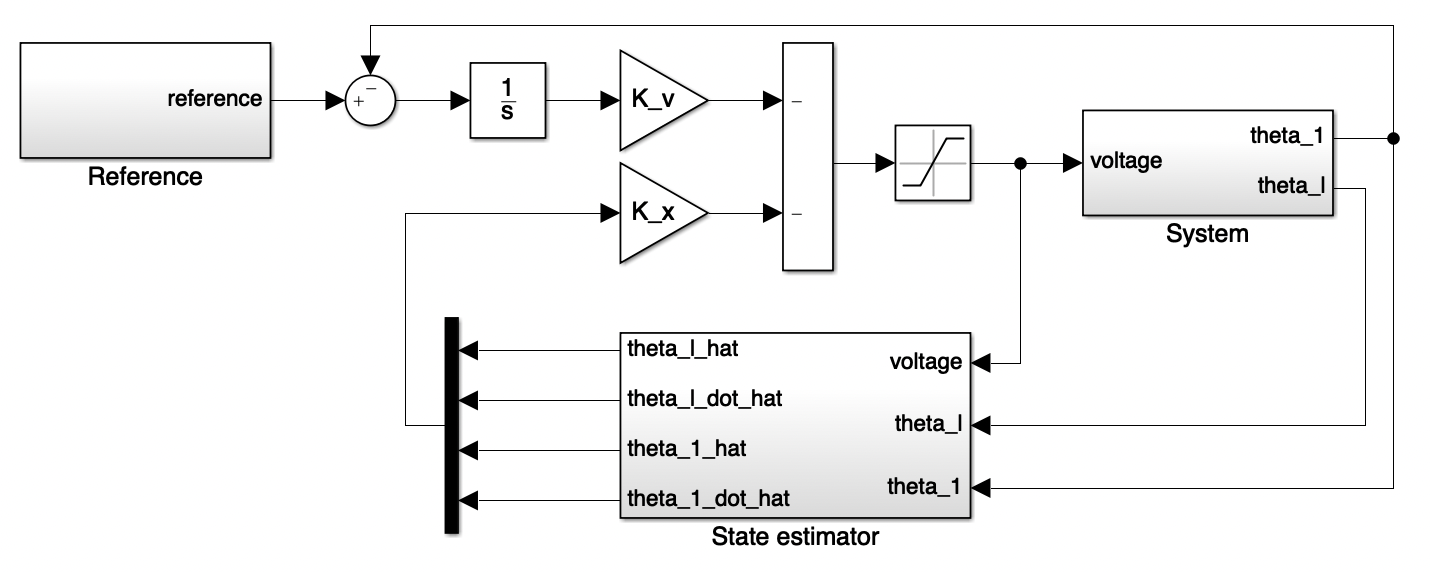
\includegraphics[width=0.7\textwidth]{pp_1dof}
	\caption{\onedof\ block-scheme, with pole placement and state reconstruction}
	\label{fig:1_dof block scheme pp + obs}
\end{figure*}

In \cref{fig:1_dof block scheme pp + obs}, the state estimator block represents either the observer or one of the Kalman Filters. 
At this point, the poles are set through the \textit{place} MATLAB function. In particular it has been decided to postpone the real poles to speed up the system, whereas concerning the complex ones it is just enhanced their damping coefficient. Turning them real would make the controller effort too aggressive, while not leading to any significant improvement in the dynamics. The placed poles and the corresponding gain~$K$ computed by the above-mentioned MATLAB function are:
\begin{equation}
	\lambda_{CL} =
	\begin{bmatrix}
		-20 \\ -50 \\ -40.1\ \bigl{(} 0.8+\sin(\arccos(0.8))i \bigr{)} \\ -40.1\ \bigl{(} 0.8-\sin(\arccos(0.8))i \bigr{)} \\-10  
	\end{bmatrix}^{T}
	\quad
	K_x =
	\begin{bmatrix}
		185.9405 \\  3.5059 \\ -125.8645 \\ 0.1222
	\end{bmatrix}^T
	\quad
	K_v =
	\begin{bmatrix}
		286.2122
	\end{bmatrix}
\end{equation}

A comparison between the same pole placement and the different state estimator is shown in figures \cref{fig:Position step response with full-state observer} and \cref{fig:Position step response with full Kalman Filter}. 
\begin{figure*}[h]
	\centering
	\begin{subfigure}{0.45\columnwidth}
		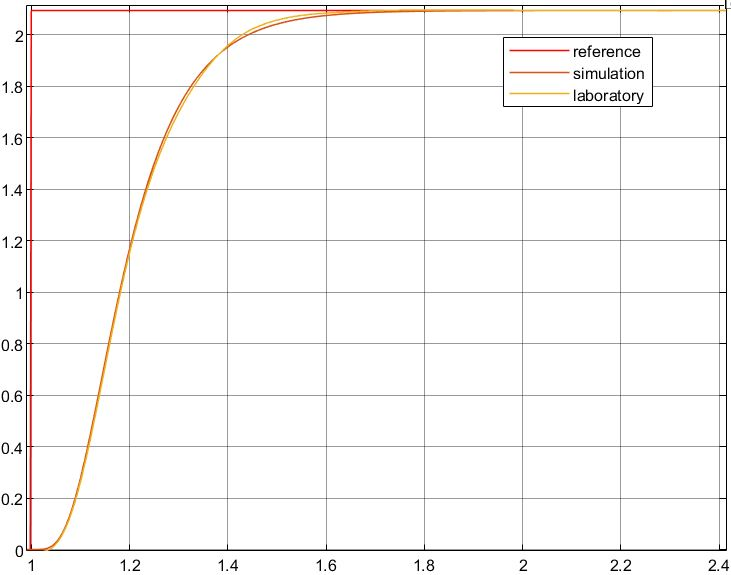
\includegraphics[scale=0.55]{response_pp_1}
		\caption{Position}
	\end{subfigure}
	\begin{subfigure}{0.45\columnwidth}
		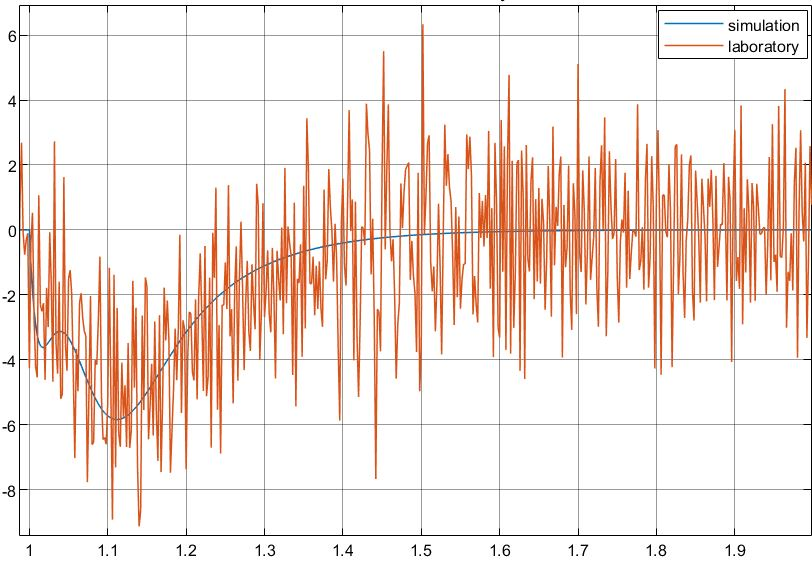
\includegraphics[scale=0.565]{voltage_pp_1}
		\caption{Voltage}
	\end{subfigure}
	\caption{Position step response with full-state observer}
	\label{fig:Position step response with full-state observer}
\end{figure*}

\begin{figure*}[h]
	\centering
	\begin{subfigure}{0.45\columnwidth}
		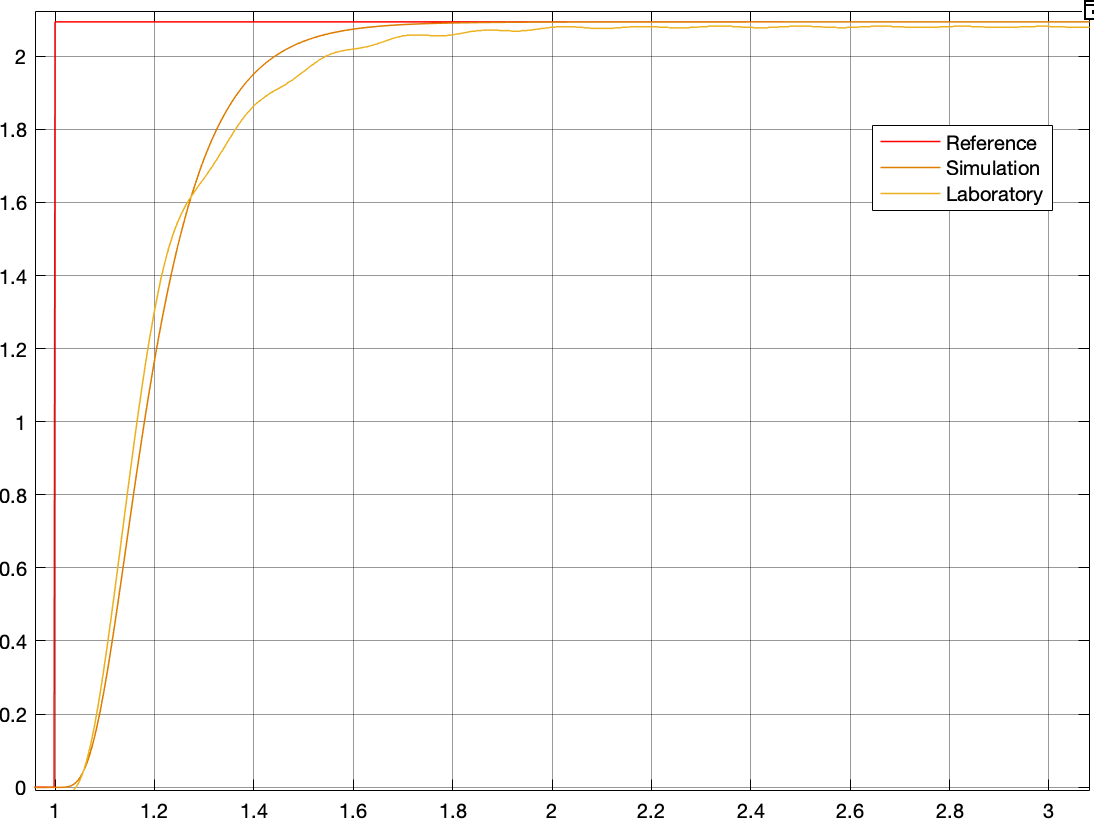
\includegraphics[scale=0.33]{kf1_pp_1}
		\caption{Position}
	\end{subfigure}
	\begin{subfigure}{0.45\columnwidth}
		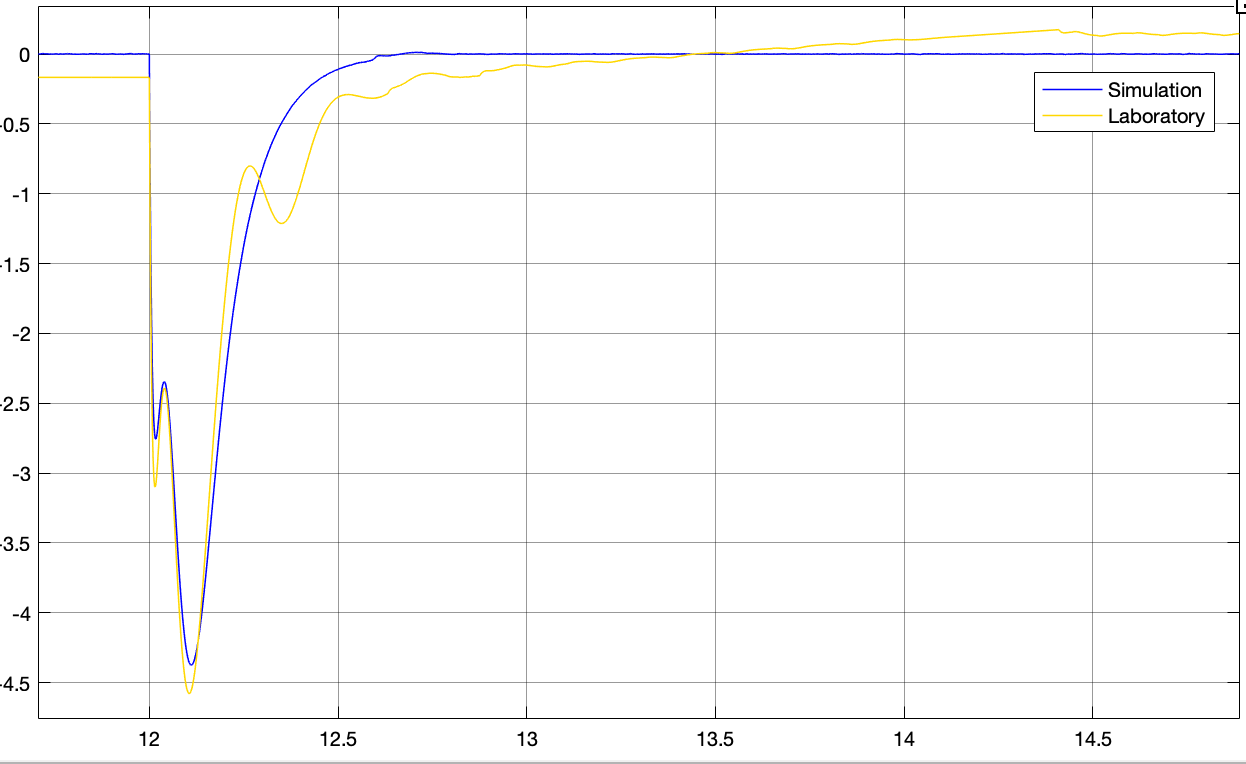
\includegraphics[scale=0.33]{kf1_pp_2}
		\caption{Voltage}
	\end{subfigure}
	\caption{Position step response with full Kalman filter (potentiometer and enconder)}
	\label{fig:Position step response with full Kalman Filter}
\end{figure*}

Regard the step response, it is possible to notice that the Kalman filter configuration is not as smooth as the observer one. This might be caused by a slower Kalman Filter state estimation. By the way, both cases are considered acceptable. On the other hand, the Kalman filter brings a significant improvement on the control action, resulting to be less noisy due to the filter robustness against the white noises.
These performances are satisfactory and a faster controller is not needed, however even better solutions will be provided later on with LQG.
\newpage
\section{\twodof\ system}
Like before, the enlarged system structure is used in order to reach the position reference. The overall enlarged state-space system and the closed control loop scheme are definitely similar to the \onedof\ case, except for the additional variables~$\theta_2$ and~$\dot\theta_2$:
\begin{center}
	$\begin{bmatrix}
		\dot{x} \\
		\dot{v}
	\end{bmatrix}
	=
	\begin{bmatrix}
		A_{sys} & 0 \\
		-C_{back} & 0
	\end{bmatrix}
	\begin{bmatrix}
		x \\
		v
	\end{bmatrix}
	+
	\begin{bmatrix}
		B_{sys} \\
		0
	\end{bmatrix}
	V$		\qquad $ C_{back} =
	\begin{bmatrix}
		0 & 0 & 0 & 0 & -1 & 0
	\end{bmatrix}$
\end{center}
\begin{figure*}[h]
	\centering
	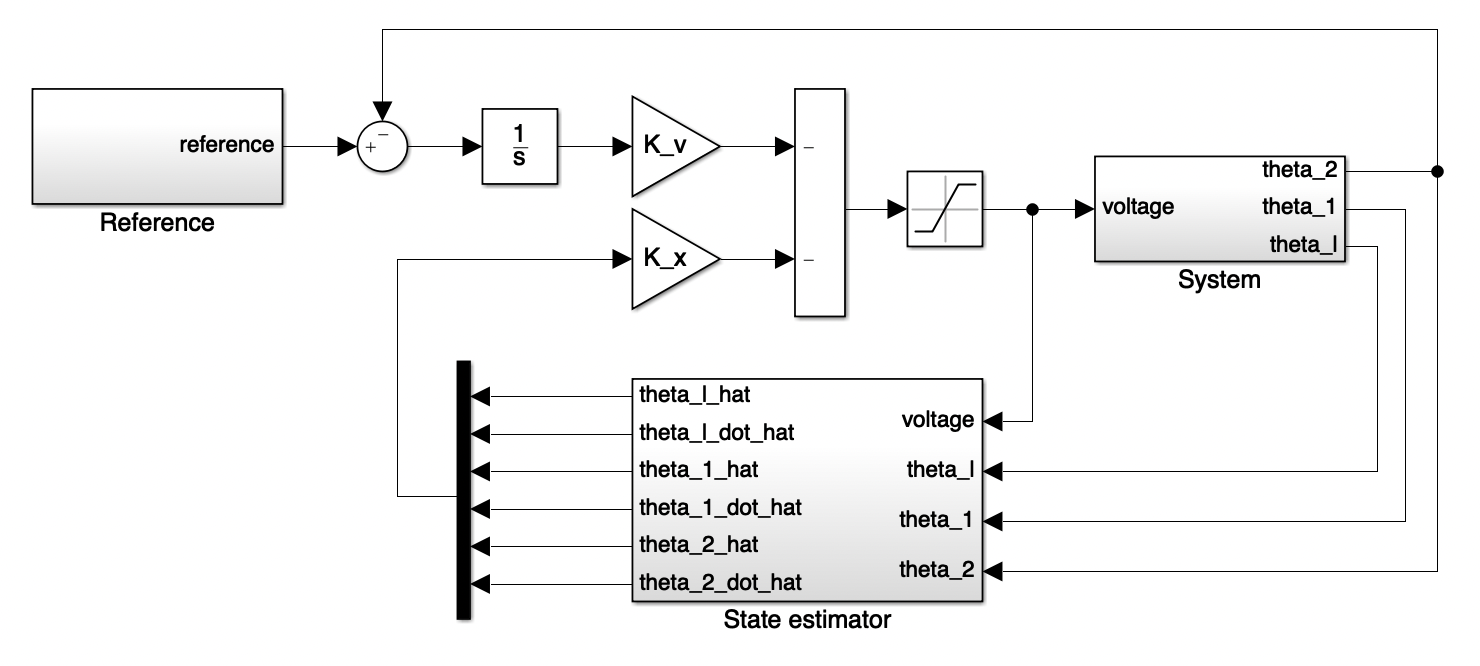
\includegraphics[width=0.7\textwidth]{pp_2dof}
	\caption{\twodof\ block-scheme, with pole placement and state reconstruction}
\end{figure*}
Also in this case, complex poles at the same frequency have been preferred over real ones; in this way only their damping has been changed:
\begin{equation}
	\lambda_{CL} =
	\begin{bmatrix}
		-20 \\ -30 \\ -24.5 \bigl{(} 0.6+\sin(\arccos(0.6))i \bigr{)} \\ -24.5 \bigl{(} 0.6-\sin(\arccos(0.6))i \bigr{)} \\
		-61.9 \bigl{(} 0.2+\sin(\arccos(0.2))i \bigr{)} \\ -61.9 \bigl{(} 0.2-\sin(\arccos(0.2))i \bigr{)} \\ -10
	\end{bmatrix}^{T}
	\quad
	K_x =
	\begin{bmatrix}
		68.1752  \\  1.1393 \\ -71.9542 \\   0.0150 \\  30.2715  \\  0.5489
	\end{bmatrix}^{T}
	\quad
	K_v =
	\begin{bmatrix}
		110.9516
	\end{bmatrix}
\end{equation}

\begin{figure*}[h]
	\centering
	\begin{subfigure}{0.5\columnwidth}
		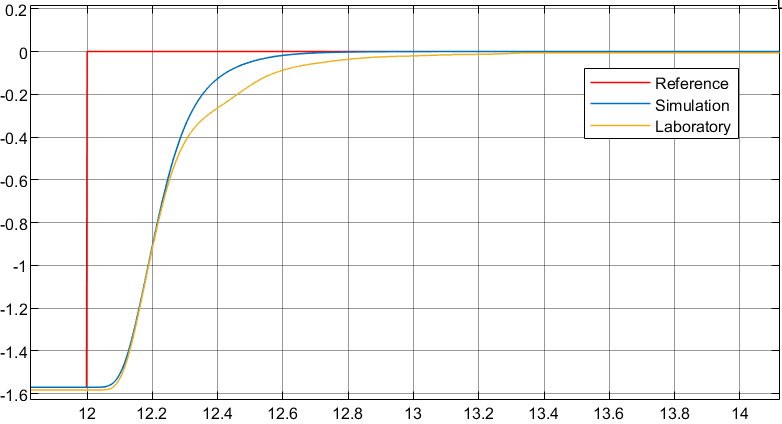
\includegraphics[scale= 0.37]{response_pp_2}
		\caption{Position}
	\end{subfigure}
	\begin{subfigure}{0.45\columnwidth}
		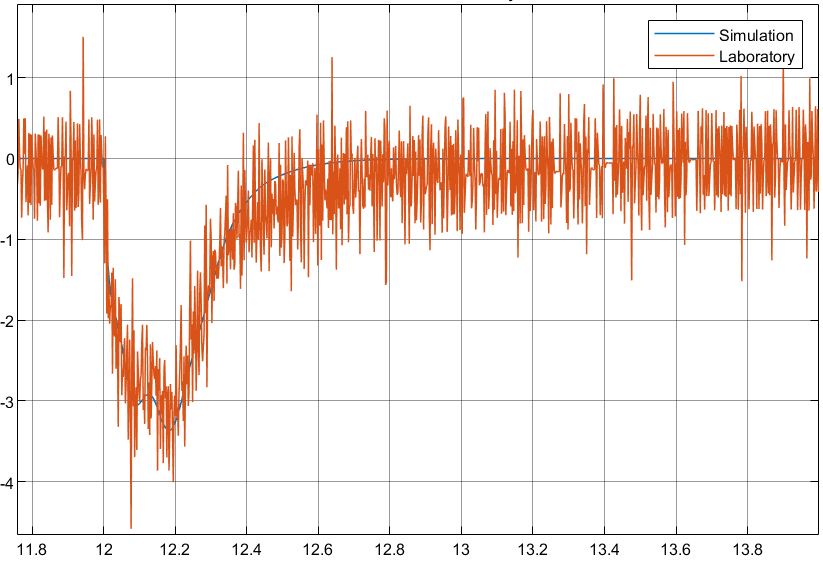
\includegraphics[scale=0.25]{voltage_pp_2}
		\caption{Voltage}
	\end{subfigure}
	\caption{Position step response with full-state observer}
\end{figure*}

\begin{figure*}[h]
	\centering
	\begin{subfigure}{0.5\columnwidth}
		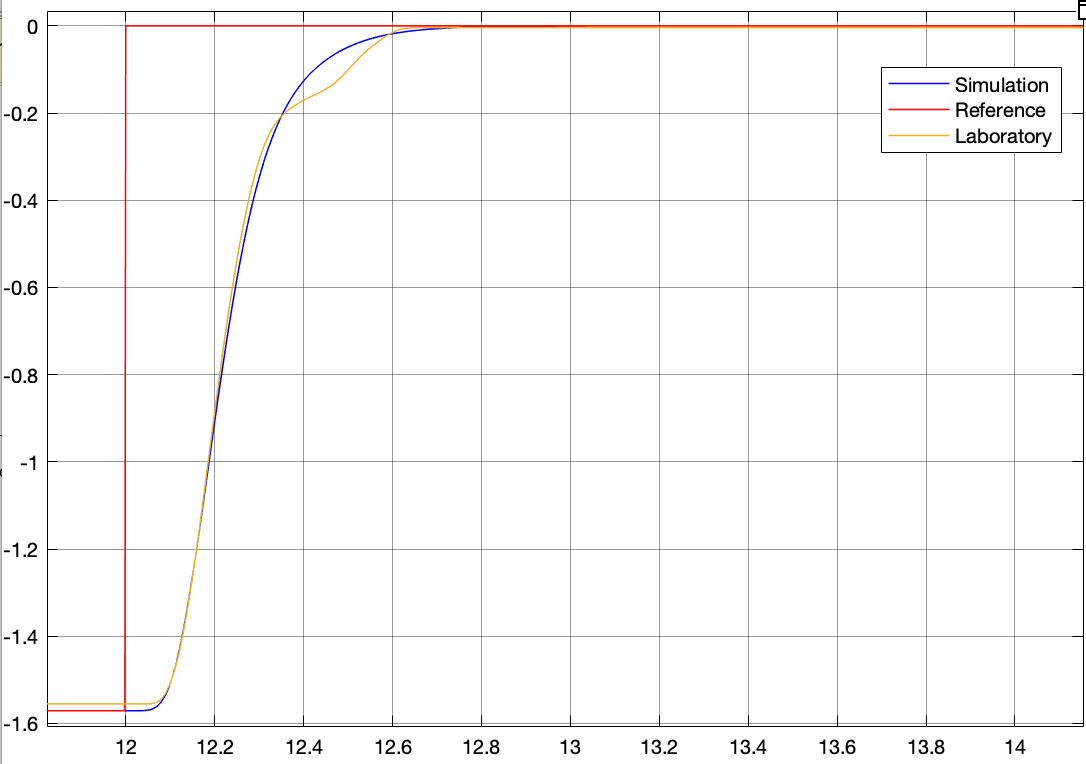
\includegraphics[scale= 0.37]{2_kf1_1}
		\caption{Position}
	\end{subfigure}
	\begin{subfigure}{0.45\columnwidth}
		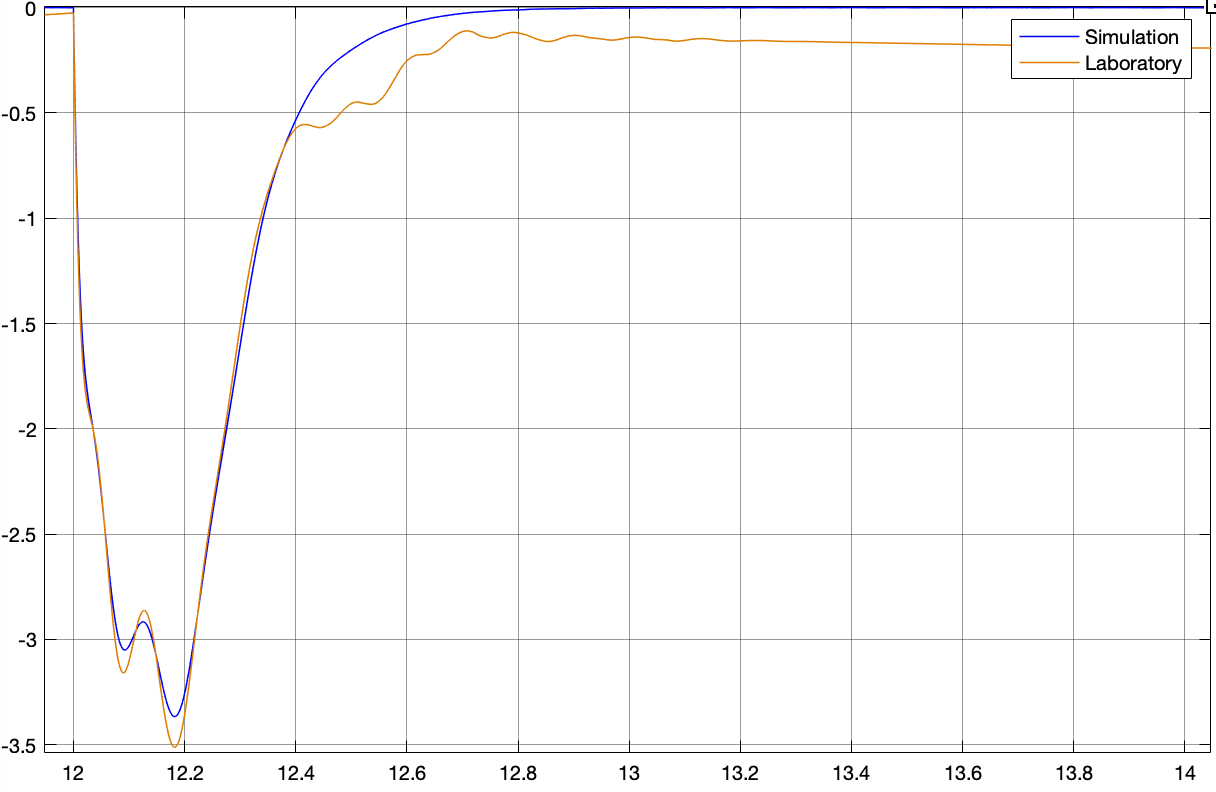
\includegraphics[scale=0.37]{2_kf1_2}
		\caption{Voltage}
	\end{subfigure}
	\caption{Position step response with full Kalman filter (potentiometer and two enconders)}
\end{figure*}

\begin{figure*}[h]
	\centering
	\begin{subfigure}{0.5\columnwidth}
		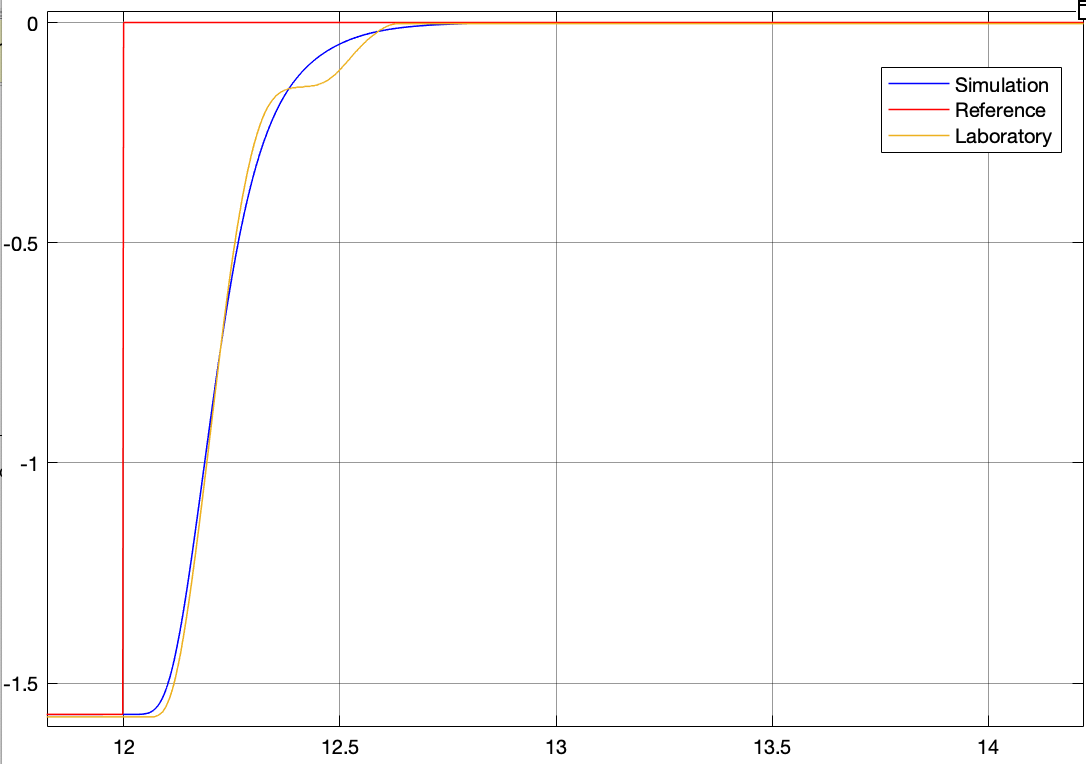
\includegraphics[scale= 0.37]{2_kf2_1}
		\caption{Position}
	\end{subfigure}
	\begin{subfigure}{0.45\columnwidth}
		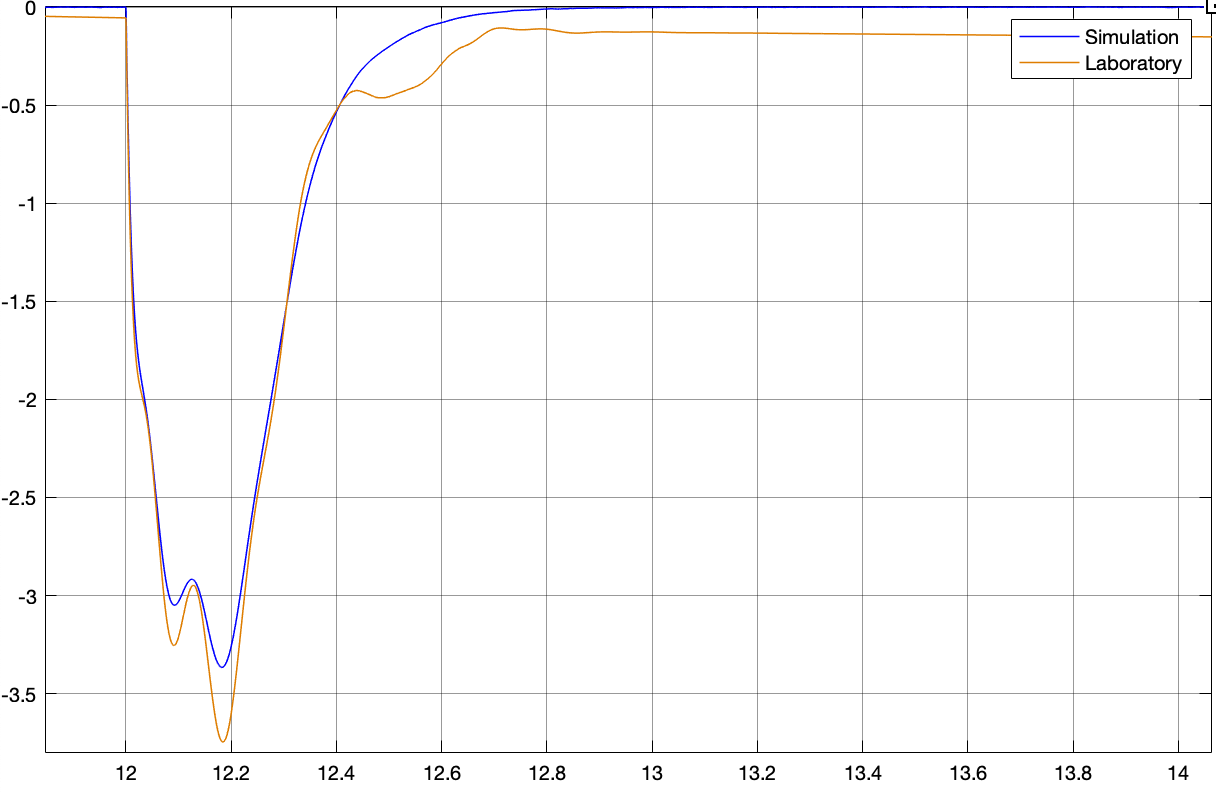
\includegraphics[scale=0.37]{2_kf2_2}
		\caption{Voltage}
	\end{subfigure}
	\caption{Position step response with Kalman filter (second mass enconder only)}
\end{figure*}
